\label{sec:experiments}

In this section, the evaluation of the instruction-based-interruption, hardware modules for post-processing, and the overall MA-Explore system are presented and analyzed.

\subsection{ Instruction-based-interruption}

The proposed interruptible is implemented and evaluated on the Xilinx ZCU102 evaluation board \cite{zcu102}. The CNN accelerator is developed based on the Xilinx AI accelerator, DPU \cite{dpu}. 

% The performance and the latency of the interruptible DPU and the not-interruptible DPU are listed in \Cref{tab:anywhere}. 
In MR-Explore, only the low-priority PR task is interruptible, and the interrupt position is unpredictable.
We record some of the interrupt locations when running MR-Explore on the interruptible DPU. The performance and the latency of the interruptible DPU and the not-interruptible DPU are listed in \Cref{tab:anywhere}. 
The execution time (Exe time) in \Cref{tab:anywhere} shows the time to complete two tasks, a interruptible PR task and a FE task.

The 'Serial' row is the baseline for executing the two tasks in serial. In serial execution, backup/recovery of data is not required. The 'CPU-like' row is the estimated result of backup/recovery all the on-chip caches for immediately interruption. The 'Pose 1,2,3' rows are the results of the DPU interrupted at different  PR positions. 'Pose 1' represents the first layers of PR network, the numbers of input channel and output channel are both $64$. The input and output shapes are both $240 \times 320$. 'Pose 2' represents the layers with moderate number of channels ($ 512 $) and data shapes ($ 60 \times 80 $). 'Pose 3' represents the last layers with many channels ($ 2048 $) and small featuremaps ($ 15 \times 20$).

DPU first calculates all channels of the output row before calculating the next rows. As the number of channels increases, the number of weights requiring recovery increases squarely. However, the size of the input data to be restored and the output results to be backed up remains basically the same.


% Table generated by Excel2LaTeX from sheet 'Sheet2'
\begin{table}[t]
  \small
  \centering
  \caption{Pref. for different interrupt positions.}
    % Table generated by Excel2LaTeX from sheet 'Sheet2'
\begin{tabular}{|c|c|c|c|c|c|}
  \hline
        & Backup  & Recovery & Exe time & Perf. & Latency \bigstrut[t]\\
        & (KB)  & (KB)  & (ms)  & Reduce & (ms) \bigstrut[b]\\
  \hline
  Pose 1 &       &       &       &       &  \bigstrut\\
  \hline
  Pose 2 &       &       &       &       &  \bigstrut\\
  \hline
  Pose 3 &       &       &       &       &  \bigstrut\\
  \hline
  CPU-Like & 4000  & 4000  &       &       & <1 \bigstrut\\
  \hline
  Serial & -     & -     &       &  baseline & - \bigstrut\\
  \hline
  \end{tabular}%
  
  
  \label{tab:anywhere}%
\end{table}%



% % Table generated by Excel2LaTeX from sheet 'Sheet1'
% \begin{table}[t]
%     \centering
%     \caption{Interrupt after complete results vs Interrupt anywhere}
% % Table generated by Excel2LaTeX from sheet 'Sheet2'
% \begin{tabular}{|c|c|c|c|c|c|}
%   \hline
%   \multicolumn{1}{|c}{} &       & \multicolumn{1}{c|}{Backup } & \multicolumn{1}{c|}{Recovery} & Exe time & Performance \bigstrut[t]\\
%   \multicolumn{1}{|c}{} &       & \multicolumn{1}{c|}{data (KB)} & \multicolumn{1}{c|}{ data (KB)} & (ms)  & Reduce \bigstrut[b]\\
%   \hline
%   \multicolumn{1}{|p{3.315em}|}{Inter } & \multicolumn{1}{p{3.69em}|}{AfterSave} &       &       &       &  \bigstrut\\
%   \cline{2-6}\multicolumn{1}{|p{3.315em}|}{position 1} & Anyware &       &       &       &  \bigstrut\\
%   \hline
%   \multicolumn{1}{|p{3.315em}|}{Inter } & \multicolumn{1}{p{3.69em}|}{AfterSave} &       &       &       &  \bigstrut\\
%   \cline{2-6}\multicolumn{1}{|p{3.315em}|}{ position 2} & Anyware &       &       &       &  \bigstrut\\
%   \hline
%   \multicolumn{1}{|p{3.315em}|}{Inter } & \multicolumn{1}{p{3.69em}|}{AfterSave} &       &       &       &  \bigstrut\\
%   \cline{2-6}\multicolumn{1}{|p{3.315em}|}{position 3} & Anyware &       &       &       &  \bigstrut\\
%   \hline
%   \multicolumn{2}{|p{7.005em}|}{CPU-Like} &       &       &       &  \bigstrut\\
%   \hline
%   \multicolumn{1}{|c}{} &       & \multicolumn{1}{c|}{Instruction} & \multicolumn{1}{c|}{Latency} & Exe time & Performance \bigstrut[t]\\
%   \multicolumn{1}{|c}{} &       & \multicolumn{1}{c|}{ (KB)} & \multicolumn{1}{c|}{(ms)} & (ms)  & Reduce \bigstrut[b]\\
%   \hline
%   \multicolumn{1}{|c|}{No} & \multicolumn{1}{p{3.69em}|}{Origin} &       &       &       & 0 \bigstrut\\
%   \cline{2-6}\multicolumn{1}{|c|}{ Interrupt} & \multicolumn{1}{p{3.69em}|}{After results} &       &       &       &  \bigstrut\\
%   \cline{2-6}      & Anyware &       &       &       &  \bigstrut\\
%   \hline
%   \end{tabular}%
  
%     \label{tab:anywhere}%
%   \end{table}%



\subsection{ Place Recognition With DPU }

In this section, we design experiments to evaluate the accuracy and efficiency of the PR network on DPU. 

\subsubsection{accuracy}

\begin{figure}[ht]
    \centering
    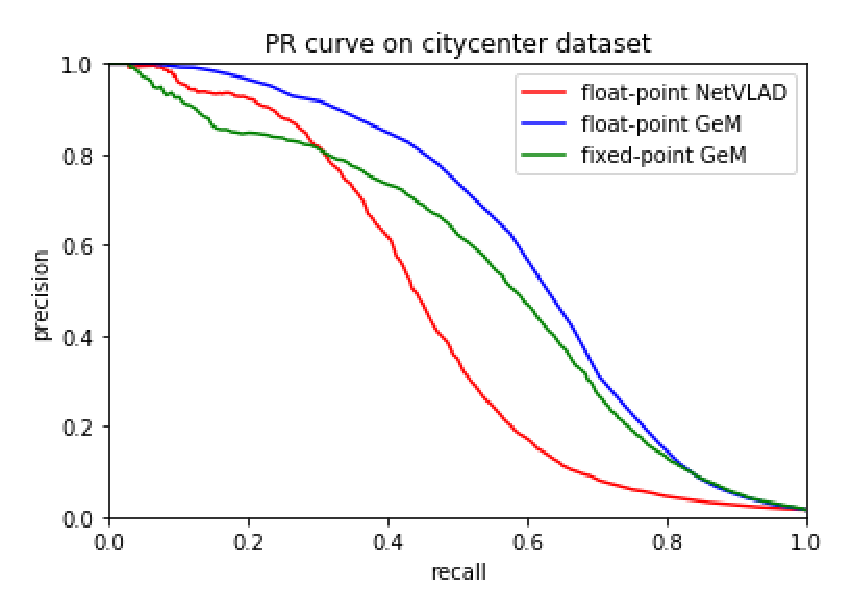
\includegraphics[width=0.8\linewidth]{fig/result.eps}
    \caption{Precision-Recall curve on Citycenter dataset}
    \label{fig:PRcurve}
\end{figure}

We want to prove two things in our experiment. 1) The GeM network used in our work outperforms other networks such as NetVLAD. 2) The quantization of GeM CNN backbone don't bring about much drop in accuracy. We test 3 networks, a) float-point GeM, b) float-point NetVLAD, c) fixed-point GeM on Citycenter dataset and draw the Precision-Recall curve. The result is shown in figure \ref{fig:PRcurve}. It's clear that float-point GeM netowrk run better than NetVLAD in all situations. After quantization, the accuracy goes down a bit, especially when precision is high. But the quantized network still outperforms NetVLAD in most cases.

\begin{figure}[ht]
  \centering
  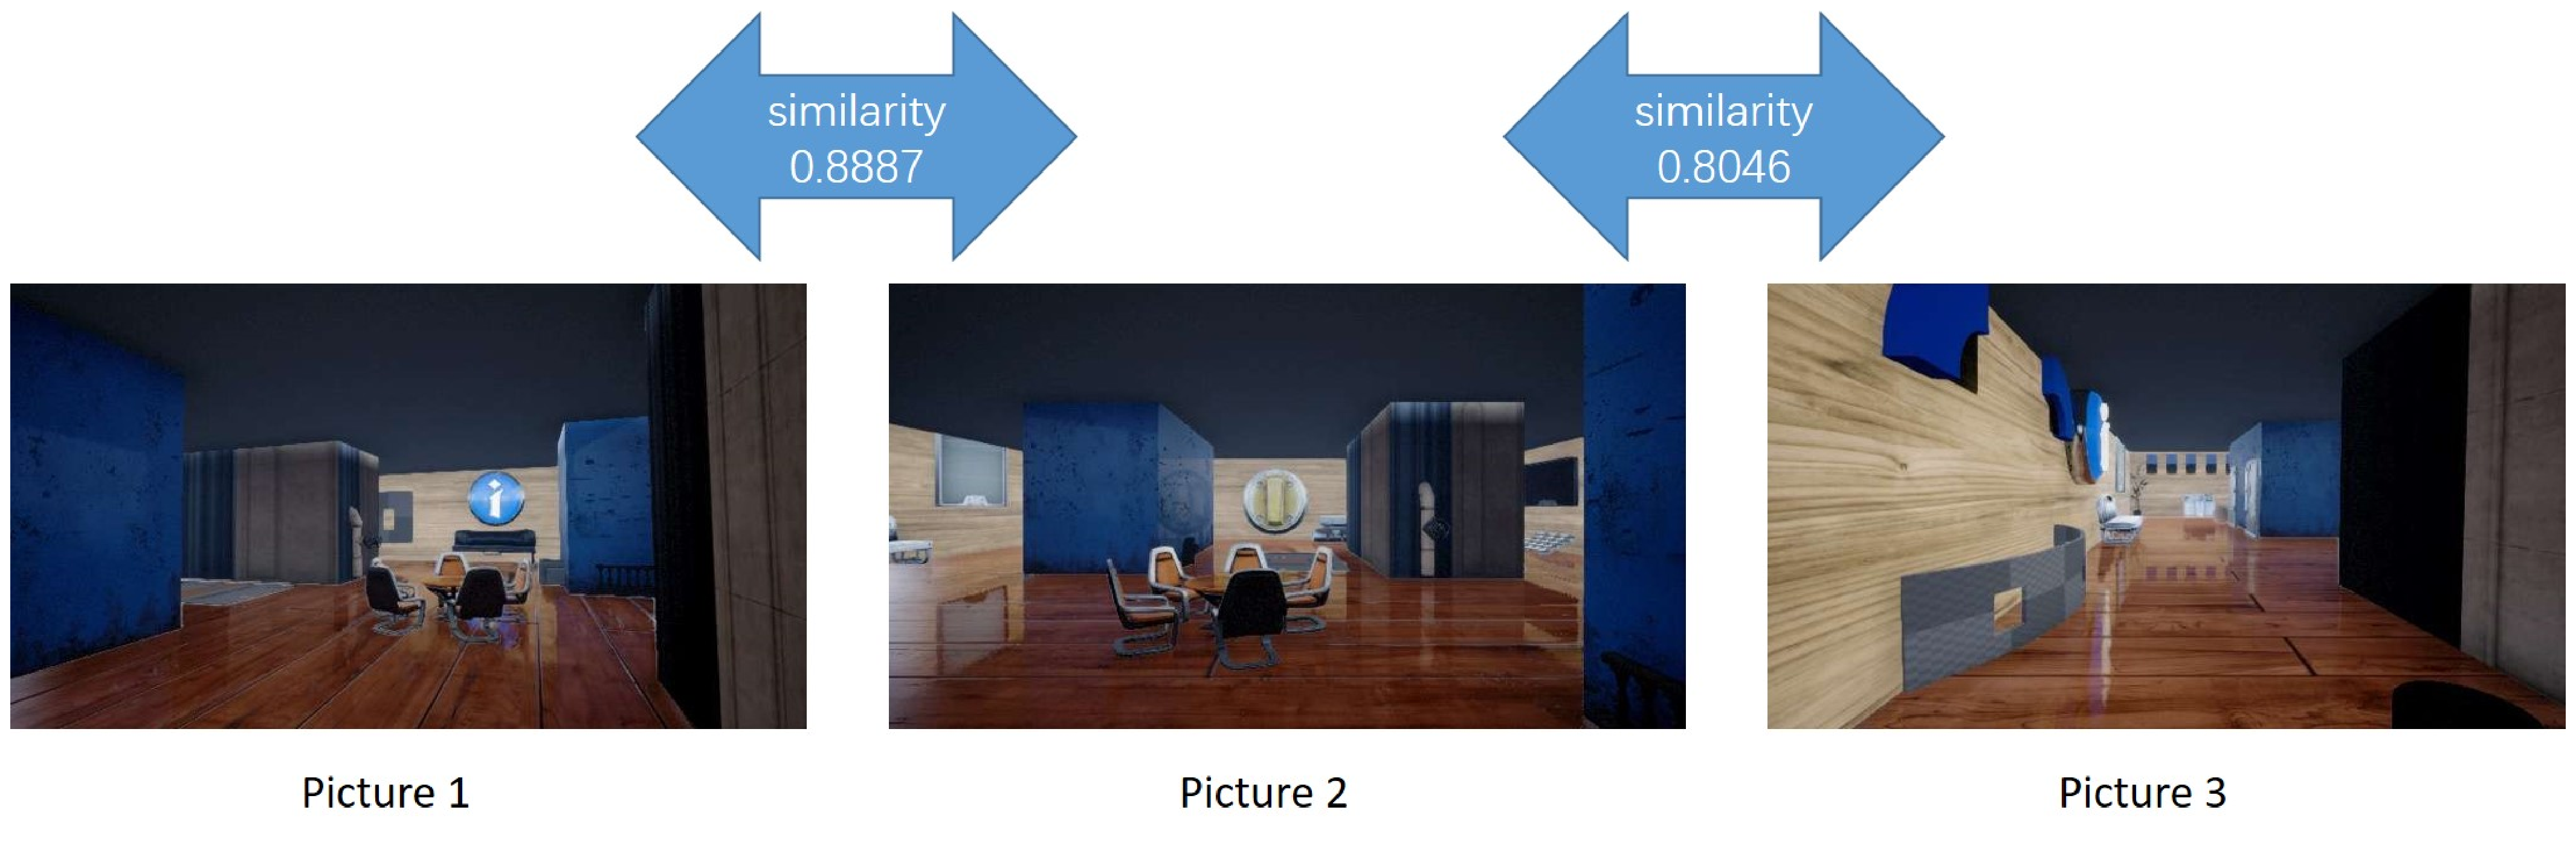
\includegraphics[width=0.8\linewidth]{fig/example.eps}
  \caption{Example of GeM performance.}
  \label{fig:gem_exp}
\end{figure}

Figure \ref{fig:gem_exp} shows an example in our similation environment. Picture 1 and Picture 2 is photoed in the same place and Picture 3 is photoed in another place. The computed similarity of Picture 1 and 2 is 0.8887, apparently larger than the similarity of Picture 2 and 3 (0.8046).

\subsubsection{efficiency}

\begin{table}
    \label{tab:gem_eff}
    \centering 
    \caption{runtime comparison of each operation in PR}
    \begin{tabular}{|c|c|c|}
				\hline
              & CPU & CPU+FPGA \\
        \hline
           &   48 ms &   42 ms \\
			  \hline
    \end{tabular}
  \end{table}

As illustrated in section \ref{sec:hardsoftcodesign}, we do optimization on GeM backend processing, i.e., the gem pooling layer. We compare running time before and after optimization, and the result is shown in table \ref{tab:gem_eff}. After optimization, the total time reduces by 12.5\%.


\subsection{ VO With DPU }

To evaluate the performance of the SuperPoint network in visual odometer, we experimented on the $TUM$ dataset. We evaluate SuperPoint against two well-known FE systems: SIFT\cite{Lowe-478} and ORB\cite{RubleeRabaud-479}. We apply the three systems to the visual odometer. We also evaluate the performance after optimization. We compute a maximum of 200 points for all systems at a $480\times640$ resolution and set $NMS=4$. We perform nearest neighbor matching from descriptors in adjacent frames with a maximum allowable distance $d_m$. $d_m$ is not same in three system because descriptors are not in the same order of magnitude. We use an OpenCV implementation (solvePnP()) with all the matches to compute the transform matrix, and use Bundle Adjustment to optimize results. All the computation of this experiment is all done on the CPU except CNN of SuperPoint. 

\begin{table}[t]
  \centering
  \caption{ Accuracy and runtime results on the TUM\cite{sturm12iros} SLAM dataset  }
  \footnotesize
  \begin{threeparttable}
% Table generated by Excel2LaTeX from sheet 'Sheet2'
\begin{tabular}{|c|c|c|c|c|} 
  \hline
        & \multirow{2}[2]{*}{$d_m$$^1$} & RPE$^2$ & ATE$^3$  & Run  \bigstrut[t]\\
        &       &  (m/s) & (m) & time(ms) \bigstrut[b]\\
  \hline
  SIFT  & 200   & 0.0319  & 0.4219 & 2397  \bigstrut\\
  \hline
  ORB   & 30    & 0.0577  & 0.6105 & 229  \bigstrut\\
  \hline
  Origin & \multirow{2}[2]{*}{0.7} & \multirow{2}[2]{*}{0.0280} & \multirow{2}[2]{*}{0.3671} & \multirow{2}[2]{*}{259} \bigstrut[t]\\
   Superpoint &       &       &       &  \bigstrut[b]\\
  \hline
  Our Fixed & \multirow{2}[2]{*}{360} & \multirow{2}[2]{*}{0.0283} & \multirow{2}[2]{*}{0.3976} & \multirow{2}[2]{*}{59} \bigstrut[t]\\
   Superpoint &       &       &       &  \bigstrut[b]\\
  \hline
  \end{tabular}%
  

\begin{tablenotes}
  \item[1] $d_m$ is the maximum allowable distance between matched descriptors.  
  \item[2] RPE is the mean Relative Pose Error to indicate the translational drift per second, the less, the better.
  \item[3] ATE is the root mean square Absolute Trajectory Error to indicate the translational drift of the entire trajectory, the less, the better.
\end{tablenotes}
    \end{threeparttable}
  \label{tab:VO}%
\end{table}%

Results are shown in \Cref{tab:VO}. In terms of accuracy, SuperPoint outperforms ORB and performs comparably to SIFT. Optimization does not introduce a large loss of accuracy. In terms of calculation speed, SuperPoint takes less time than Sift, and is equivalent to Orb. After optimization, the running speed is increased by $4\times$, making real-time processing possible.

\begin{table}[t]
  \centering
  \caption{runtime Comparison of each operation}
% Table generated by Excel2LaTeX from sheet 'Sheet2'
\begin{tabular}{|c|c|c|c|c|}
  \hline
             &    softmax &        NMS &       rank &  normalize \bigstrut\\
  \hline
         CPU &       31ms &       27ms &       0.97ms &       42ms \bigstrut\\
  \hline
    CPU+FPGA &     1.97ms &      0.7ms &     0.12ms &     1.44ms \bigstrut\\
  \hline
  \end{tabular}  
  
  \label{tab:optimization}%
\end{table}%

We compare the running time of each operation in SuperPoint before and after the optimization. Results are shown in \Cref{tab:optimization}. The running time of each operation is reduced by more than $20\times$. There is a certain gap between the experimental results of the acceleration effect and the theoretical derivation in \Cref{subsec:FEopt}. The possible reason is that the CPU needs time to schedule the FPGA accelerator.

\subsection{ ROS based MA-Explore }

\subsubsection { Hardware Resources Utilization }

The proposed ROS based MA-Explore is inplemented and evaluated on the ZCU102 evaluate board \cite{zcu102}, which is provied by Xilinx. The CNN backbone is calculated by Xilinx AI accelerator, DPU\cite{dpu}, which is a hardware IP implemented on the FPGA side of ZCU102 (Programable logic, PL side). The FE and the PR post-processing steps run on our proposed accelerators, also on the PL side. The PL side has 3 clock frequencies. The DPU are running at 300MHz. The accelerator for FE are running at 200MHz and the accelerator for PR are running at 100MHz.

\Cref{tab:hardware} shows the hardware resources utilization of DPU and our proposed accelerators. About 48\% of on-board hardware resources are used by DPU. Our proposed accelerators only use a small amount of hardware resources compared with the DPU.
% Table generated by Excel2LaTeX from sheet 'Sheet1'
\begin{table}[t]
  \centering
  \caption{Hardware comsumption of the proposed hardware}
% Table generated by Excel2LaTeX from sheet 'Sheet1'
\begin{tabular}{|c|c|c|c|c|}
  \hline
        & $\sharp$ DSP & $\sharp$ LUT & $\sharp$ FF & $\sharp$ BRAM \bigstrut\\
  \hline
  On-Board Resource &   2520   &  274080      &  548160     & 912 \bigstrut\\
  \hline
  DPU &   1282   &  74569      &   171416    & 499 \bigstrut\\
  \hline
  FE & 25      &  17573     &   29115    & 10 \bigstrut\\
  \hline
  PR & 109      &  7169     &   5601    & 11.5 \bigstrut\\
  \hline
  \end{tabular}%
  
  
  
  
  \label{tab:hardware}%
\end{table}%